    \subsection*{Review: LLC as Neuron}
    
        Remember that we can represent our LLC as a \textbf{neuron}: this could give us the first idea for how to train our \textbf{neural network}!
        
        \begin{figure}[H]
            \centering
            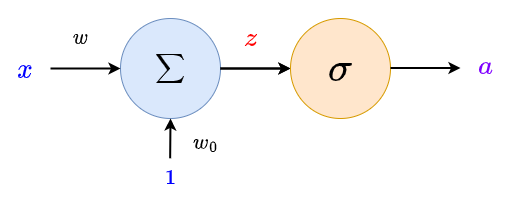
\includegraphics[width=80mm,scale=0.4]{images/nn_1_5_images/llc_as_neuron.png}
        \end{figure}
        
        As usual, our first unit $\sum$ is our \textbf{linear} component. The output is $z$, nothing different from before with LLC.
            \note{Remember that $x$ is a whole vector of values, which we've condensed into one variable.}
        
        The \textbf{output} of $\sigma$, which we wrote before as $g$, is now $a$.
        
        Something we neglected before: this diagram is \textbf{missing} the \textbf{loss function}. Let's create a small unit for that. 
        
        $\loss(a,y)$ has \textbf{two} inputs: our predicted value $a$, and the correct value $y$. 
        
        \begin{figure}[H]
            \centering
            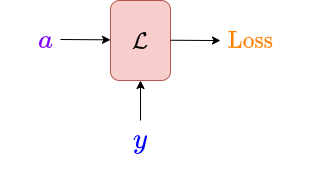
\includegraphics[width=60mm,scale=0.4]{images/nn_1_5_images/loss_unit.png}
            \caption*{We have two inputs to our loss function.}
        \end{figure}
        
        We \textbf{combine} these into a single unit to get:
        
        \begin{figure}[H]
            \centering
            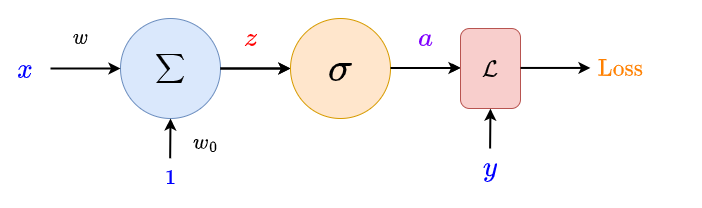
\includegraphics[width=90mm,scale=0.4]{images/nn_1_5_images/llc_as_neuron_loss.png}
        \end{figure}
        
        Our full unit!
        
    \secdiv
    
    \subsection*{LLC Forward-Pass}
    
        Now, we can do gradient descent like before. We want to get the effect our \textbf{weight} has on our \textbf{loss}.
        
        But, this time, we'll pair it with a \textbf{visual} that is helpful for understanding how we \textbf{train} neural networks. 
        
        First, one important consideration:
        
        As we saw above, the \textbf{gradient} we get might rely on $z$, $a$, or $\loss(a,y)$. So, before we do anything, we have to \textbf{compute} these values.
        
        Each step \textbf{depends} on the last: this is what the \textbf{forward} arrows represent. We call this a \textbf{forward pass} on our neural network.\\
        
        \begin{definition}
            A \vocab{forward pass} of a neural network is the process of sending information "\gren{forward}" through the neural network, starting from the \purp{input}.
            
            This means the \purp{input} is fed into the \gren{first} layer, and that output is fed into the \gren{next} layer, and so on, until we reach our \purp{final} result and \purp{loss}.
        \end{definition}
        
        \miniex If we had 
        
        \begin{itemize}
            \item $\blu{f}(\red{x}) = \red{x}+2$
            
            \item $\org{g}(\blu{f}) = 3\blu{f}$
            
            \item $h(\org{g}) = \sin(\org{g})$
        \end{itemize}
        
        Then, a forward pass with the input $x=10$ would have us go function-by-function:
        
        \begin{itemize}
            \item $\blu{f}(\red{10}) = \red{10}+2$
            
            \item $\org{g}(\blu{f}) = 3 \cdot \blu{12}$
            
            \item $h(\org{g}) = \sin(\org{36})$
        \end{itemize}
        
        So, by "forward", we mean that we apply each function, one after another.
        
        In our case, this means computing $z$, $a$, and $\loss(a,y)$.
        
    \secdiv
    
    \subsection*{LLC Back-propagation}
    
        Now that we have all of our values, we can get our gradient. Let's \textbf{visualize} this process.
        
        \begin{figure}[H]
            \centering
            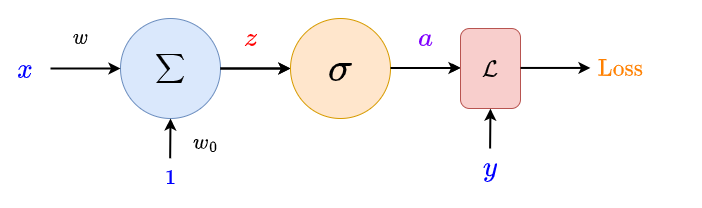
\includegraphics[width=90mm,scale=0.4]{images/nn_1_5_images/llc_as_neuron_loss.png}
        \end{figure}
        
        We want to link $\loss$ to $w$. In order to do that, we need to \textbf{connect} each thing in between.
        
        This lets us \textbf{combine} lots of simple \textbf{links} to get our more complicated result.
            \note{We can also call this "chaining together" lots of derivatives.}
            
        Loss is what we really care about. So, what is the loss directly \textbf{connected} to? The \textbf{activation}, $a$.
        
        \begin{figure}[H]
            \centering
            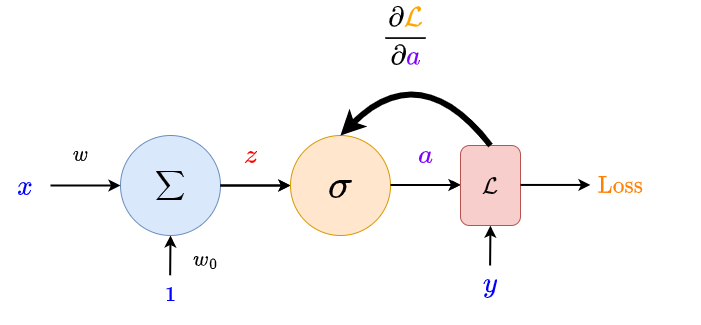
\includegraphics[width=90mm,scale=0.4]{images/nn_1_5_images/llc_backprop_1.png}
        \end{figure}
        
        So, our $\sigma$ unit has information about the derivative that comes after it: the \textbf{loss} derivative
        
        \begin{equation}
            \overbrace{
                \pderiv {\pur{\loss}} {\blu{a}} 
            }^{\text{Loss unit}} 
        \end{equation}
        
        And what is that connected to? The \textbf{pre-activation} $z$:
        
        \begin{figure}[H]
            \centering
            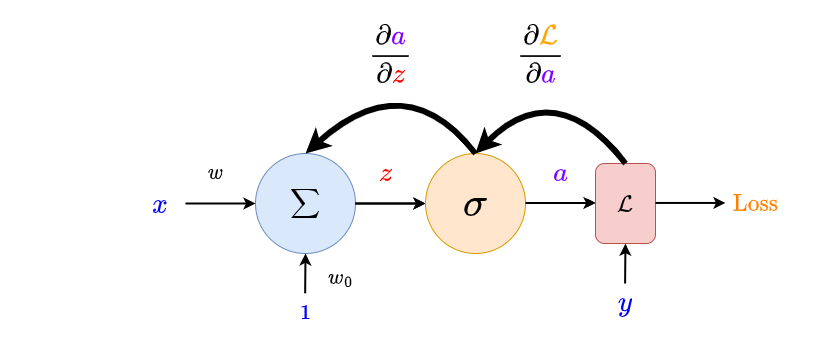
\includegraphics[width=100mm,scale=0.4]{images/nn_1_5_images/llc_backprop_2.png}
        \end{figure}
        
        Now, our $\sum$ unit has information about both the \textbf{loss} derivative and the $\sigma$ derivative:
        
        \begin{equation}
            \overbrace{
                \pderiv {\pur{\loss}} {\blu{a}} 
            }^{\text{Loss unit}}
            \cmul
            \overbrace{
                \pderiv {\blu{a}}     {\red{z}}
            }^{\text{Activation function}}
        \end{equation}
       
        
        And finally, we've reached $w$:
        
        \begin{figure}[H]
            \centering
            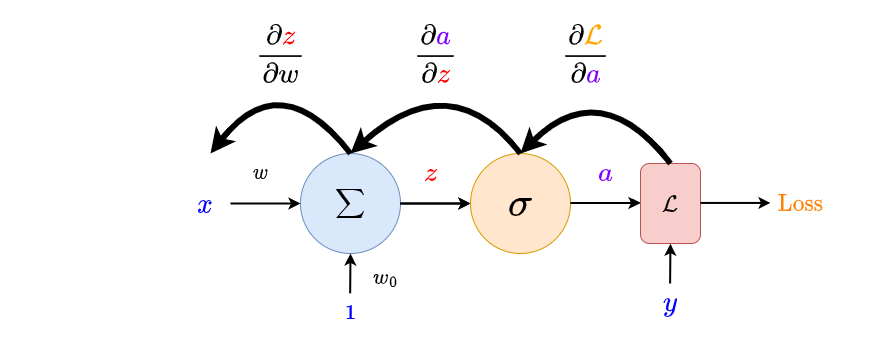
\includegraphics[width=110mm,scale=0.4]{images/nn_1_5_images/llc_backprop_3.png}
        \end{figure}
        
        And, we built our chain rule! This contains the \textbf{information} of the derivatives from \textbf{every} unit.
        
        \begin{equation}
            \pderiv {\pur{\loss}} {w} 
            =
            \overbrace{
                \pderiv {\pur{\loss}} {\blu{a}} 
            }^{\text{Loss unit}}
            \cmul
            \overbrace{
                \pderiv {\blu{a}}     {\red{z}}
            }^{\text{Activation}}
                \cmul
            \overbrace{
                \pderiv {\red{z}}     {w}
            }^{\text{Linear subunit}}
        \end{equation}
        
        Moving backwards like this is called \textbf{back-propagation}.\\
        
        \begin{definition}
            \vocab{Back-propagation} is the process of moving "\gren{backwards}" through your network, starting at the \purp{loss} and moving back layer-by-layer, and gathering terms in your \purp{chain rule}.
            
            We call it "\purp{propagation}" because we send backwards the \gren{terms} of our chain rule about later derivatives.
            
            An \gren{earlier} unit (closer to the "left") has all of the \purp{derivatives} that come after (to the "right" of) it, along with its own term.
        \end{definition}
        
    \secdiv
    
    \subsection*{Summary of neural network gradient descent: a high-level view}
    
        So, with just this, we have built up the basic idea of how we \textbf{train} our model: now that we have the gradient, we can do \textbf{gradient descent} like we normally do!
            \note{This summary covers some things we haven't fully discussed. We'll continue digging into the topic!}\\
        
        \begin{concept}
            We can do \vocab{gradient descent} on a \vocab{neural network} using the ideas we've built up:
            
            \boxdiv
            
            \begin{itemize}
                \item Do a \vocab{forward pass}, where we compute the value of each \gren{unit} in our model, passing the information \purp{forward} - each layer's \textbf{output} is the next layer's \textbf{input}.
                    \begin{itemize}
                        \item We finish by getting the \purp{loss}.
                    \end{itemize}
                    
            \boxdiv
                    
                \item Do \vocab{back-propagation}: build up a \purp{chain rule}, starting at the \purp{loss} function, and get each unit's \gren{derivative} in \purp{reverse order}.
                    \begin{itemize}
                        \item \purp{Reverse} order: if you have 3 layers, you want to get the 3rd layer's \gren{derivatives}, then the 2nd layer, then the 1st.
                        
                        \item \purp{Each weight} vector has its own \gren{gradient}: we'll deal with this later, but we need to calculate one for each of them.
                    \end{itemize}
                    
            \boxdiv
                
                \item Use your chain rule to get the \purp{gradient} $\pderiv{\loss}{w}$ for your \gren{weight} vector(s). Take a \vocab{gradient descent} step.
                
                \item \vocab{Repeat} until satisfied, or your model \purp{converges}.
            \end{itemize}
        \end{concept}
        
        
        